% Latex template: mahmoud.s.fahmy@students.kasralainy.edu.eg
% For more details: https://www.sharelatex.com/learn/Beamer

\documentclass{beamer}					% Document class

\setbeamertemplate{footline}[text line]{%
  \parbox{\linewidth}{\vspace*{-8pt}The variational autoencoder\hfill\insertshortauthor\hfill\insertpagenumber}}
\setbeamertemplate{navigation symbols}{}

\usepackage[english]{babel}				% Set language
\usepackage[utf8x]{inputenc}			% Set encoding

\mode<presentation>						% Set options
{
  \usetheme{default}					% Set theme
  \usecolortheme{default} 				% Set colors
  \usefonttheme{default}  				% Set font theme
  \setbeamertemplate{caption}[numbered]	% Set caption to be numbered
}

% Uncomment this to have the outline at the beginning of each section highlighted.
%\AtBeginSection[]
%{
%  \begin{frame}{Outline}
%    \tableofcontents[currentsection]
%  \end{frame}
%}

\usepackage{graphicx}					% For including figures
\usepackage{booktabs}					% For table rules
\usepackage{hyperref}					% For cross-referencing

\title{The variational autoencoder}	% Presentation title
\author{Clayton W. Seitz}								% Presentation author
\date{\today}									% Today's date

\begin{document}

% Title page
% This page includes the informations defined earlier including title, author/s, affiliation/s and the date
\begin{frame}
  \titlepage
\end{frame}

% Outline
% This page includes the outline (Table of content) of the presentation. All sections and subsections will appear in the outline by default.


% The following is the most frequently used slide types in beamer
% The slide structure is as follows:
%
%\begin{frame}{<slide-title>}
%	<content>
%\end{frame}



%\begin{frame}{Variational autoencoders (VAEs)}
%A variational solution to generative modeling
%
%\begin{center}
%\begin{figure}
%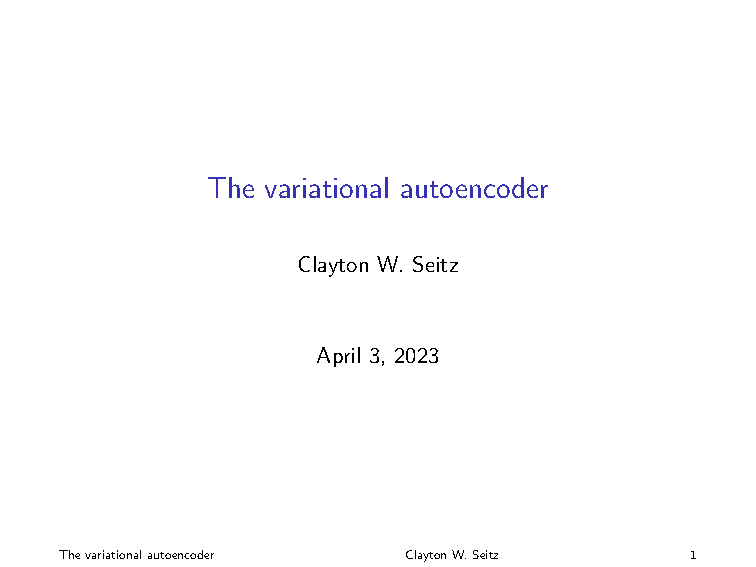
\includegraphics[width=0.9\textwidth]{vae}
%\caption{\textbf{Variational autoencoder architecture} Taken from Lopez 2020 in EMBO}
%\end{figure}
%\end{center}
%\end{frame}


\begin{frame}{Variational Bayes}

The variable $\mathbf{x}$ has a latent representation or code $\mathbf{z}$. We often say that $\mathbf{z}$ is the \emph{causal source} of $\mathbf{x}$. The distribution we are after is the \emph{evidence} in Bayes rule $P(\mathbf{x})$

\begin{equation*}
P(\mathbf{x}) = \frac{P_{\Phi}(\mathbf{x|z})P_{\Omega}(\mathbf{z})}{Q_{\Psi}(\mathbf{z|x})}
\end{equation*}

It is common to take $P_{\Omega}(\mathbf{z})$ to be Gaussian. We then try find the model parameters $\Theta = (\Phi,\Psi)$ that maximize the likelihood of the observed data:

\begin{equation*}
\Theta^{*} = \underset{\Theta}{\mathrm{argmin}} -\log P(\mathbf{x}_{\textrm{obs}}) 
\end{equation*}


\end{frame}

\begin{frame}{Computing the evidence}

We can alternatively write the evidence as

\begin{align*}
P(\mathbf{x}) &= \int P_{\Omega}(\mathbf{z})P_{\Phi}(\mathbf{x|z})d\mathbf{z}\\
&= \int P_{\Omega}(\mathbf{z})P_{\Phi}(\mathbf{x|z})\frac{P_{\Psi}(\mathbf{z|x})}{P_{\Psi}(\mathbf{z|x})}d\mathbf{z}\\
&= \mathbb{E}_{\mathbf{z}\sim P_{\Psi}(\mathbf{z|x})} \frac{P_{\Omega}(\mathbf{z})P_{\Phi}(\mathbf{x|z})}{P_{\Psi}(\mathbf{z|x})}
\end{align*}

We call $\Psi$ and $\Phi$ the encoder and decoder, respectively

\end{frame}

\begin{frame}{The evidence lower bound (ELBO)}

\begin{align*}
\log P(\mathbf{x}) &= \log \;\mathbb{E}_{\mathbf{z}\sim P_{\Psi}(\mathbf{z|x})} \frac{P_{\Omega}(\mathbf{z})P_{\Phi}(\mathbf{x|z})}{P_{\Psi}(\mathbf{z|x})}\\
&\geq \mathbb{E}_{\mathbf{z}\sim  P_{\Psi}(\mathbf{z|x})} \log \;\frac{P_{\Omega}(\mathbf{z})P_{\Phi}(\mathbf{x|z})}{P_{\Psi}(\mathbf{z|x})}
\end{align*}

\begin{equation*}
-\log P(\mathbf{x}) \leq \mathbb{E}_{\mathbf{z}\sim P_{\phi}(\mathbf{z|x})} \log \frac{P_{\Psi}(\mathbf{z|x})}{P_{\Omega}(\mathbf{z})} - \log P_{\Phi}(\mathbf{x|z})
\end{equation*}


\end{frame}

\begin{frame}{The ELBO objective}


\begin{align*}
\Theta^{*} &= \underset{\Phi,\Psi}{\mathrm{argmin}} \;\;\mathbb{E}_{\mathbf{x}\sim \mathrm{Pop},\; \mathbf{z}\sim P_{\Psi}(\mathbf{\mathbf{z}|\mathbf{x}})} \log \frac{P_{\Psi}(\mathbf{z|x})}{P_{\Omega}(\mathbf{z})} - \log P_{\Phi}(\mathbf{x|z})\\
&= \underset{\Phi,\Psi}{\mathrm{argmin}} \;\; D_{\mathrm{KL}}\left(P_{\Psi}||P_{\Omega}\right) - \mathbb{E}_{\mathbf{x}\sim \mathrm{Pop},\;\mathbf{z}\sim P_{\Psi}(\mathbf{\mathbf{z}|\mathbf{x}})}  \log P_{\Phi}(\mathbf{x|z})
\end{align*}

\vspace{0.1in}
The first term is a \textbf{rate term} to be minimized and the second a \textbf{reconstruction term} to be maximized

\end{frame}


%\begin{frame}{Applying deep generative models to biological data}
%\begin{figure}
%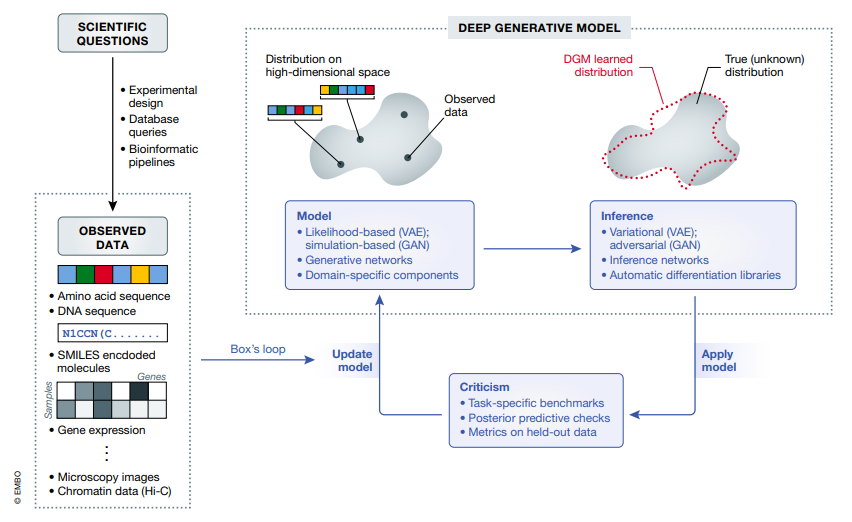
\includegraphics[height=65mm, width=105mm]{dbm}
%\end{figure}
%\end{frame}


\section{References}

% Adding the option 'allowframebreaks' allows the contents of the slide to be expanded in more than one slide.
\begin{frame}[allowframebreaks]{References}
	\tiny\bibliography{references}
	\bibliographystyle{apalike}
\end{frame}

\end{document}